% HW2 high dimensional data

\documentclass[12pt, leqno]{article}
\usepackage{amsfonts, amsmath, amssymb}
\usepackage{amsthm}
\usepackage{mathtools}
\usepackage{fancyhdr}
\usepackage{hyperref}
\usepackage{graphicx}
\usepackage{caption}
\usepackage{subcaption}
\usepackage{float}
\usepackage{mathrsfs}
\usepackage{array} 
\usepackage{rotating}
%\usepackage{babel}
\providecommand{\abs}[1]{\lvert#1\rvert}
\providecommand{\norm}[1]{\lVert#1\rVert}
\newcommand{\macheps}{\epsilon_{\mbox{\scriptsize mach}}}
\let\oldhat\hat
\renewcommand{\vec}[1]{\mathbf{#1}}
\renewcommand{\hat}[1]{\oldhat{{#1}}}
\def\rp{\ensuremath \mathbb{R}^p}
\def\rpp{\ensuremath \mathbb{R}^{p \times p}}
\def\s{\ensuremath\Sigma}
\def\om{\ensuremath\Omega}
\def\pd{\ensuremath\mathbb{P}^+}
\def\pg{\ensuremath\mathbb{P}_{{G}}}
\def\E{\ensuremath\mathbb{E}}
\def\normdist[#1]#2{\ensuremath \sim \mathcal{N} (#1,#2) }
\def\ndist1{\ensuremath \sim \mathcal{N}  (\mu, \sigma)}
\def\ndistvec{\ensuremath \sim \mathcal{N}_p ( {\mu},  {\Sigma})}
\def\lra{\ensuremath\Leftrightarrow}
\def\stackrel#1#2{\mathrel{\mathop{#2}\limits^{#1}}}
\newcommand\ind{\protect\mathpalette{\protect\independenT}{\perp}}
\def\independenT#1#2{\mathrel{\rlap{$#1#2$}\mkern2mu{#1#2}}}
\makeatletter
\newtheorem{thm}{Theorem}[]
\newtheorem{lemma}{Lemma}[]
\newtheorem{defn}[thm]{Definition}
\newcommand{\sign}{\mathrm{sign}}
\newcommand{\distas}[1]{\mathbin{\overset{#1}{\kern\z@\sim}}}%
\newsavebox{\mybox}\newsavebox{\mysim}
\newcommand{\dist}[1]{%
  \savebox{\mybox}{\hbox{\kern3pt$\scriptstyle#1$\kern3pt}}%
  \savebox{\mysim}{\hbox{$\sim$}}%
  \mathbin{\overset{#1}{\kern\z@\resizebox{\wd\mybox}{\ht\mysim}{$\sim$}}}%
}
\makeatother

\begin{document}
\pagestyle{fancy}
\lhead{TA,RB,SR,AS}
\rhead{STA7934}

\begin{center}
{\large {\bf Homework 2 - Analysis of High Dimensional Data}} \\
{\it{Tavis Abrahamsen, Ray Bai, Syed Rahman and Andrey Skripnikov}} \\
\end{center}

\paragraph{Logistic Regression with Lasso Penalty} Consider a classification problem, where the response is
binary $y \in \{0,1\}$ and the predictor variables numerical. Generate
a design matrix $X$ of size 5,000 by 300
 (i.e. 5,000 observations and 300 variables). Generate the corresponding response $y$ by selecting an appropriate coefficient vector $\beta$ and adding a noise term.

Consider a model where the true coefficient vector has only 20 non-zero
elements and another with 75 non-zero elements. Devise a sub-gradient
based algorithm (soft-thresholding) to solve the problem, where the Gram matrix $X'X$ is well-conditioned.

Compare the performance of your algorithm for a grid of the tuning parameter $\lambda$.

\paragraph{} We are interested in solving the
logistic regression from last time with a $lasso$ penalty added
on. Recall that last time our objective was to minimize the negative log likelihood 
\[
-l(\beta) = -\sum_{i=1}^{n} [y_i \log (\pi_i)+ (1-y_i) \log (1-\pi_i)]
\]
where 
\[
\log (\frac{\pi_i}{1-\pi_i}) = {x_i' \beta}.
\]
While $\nabla (-l(\beta)) = 0$ has no closed form solutions, it is a convex function as we
showed last time and hence we can use the gradient descent algorithm 
\[
\beta^{k+1} = \beta^{k} - \alpha^k \nabla (-l(\beta^k))
\]
where $\alpha^k$ is a suitably chosen stepsize and $-\nabla l(\beta^k) = -X'(y-\frac{e^{X \beta}}{1+e^{X
    \beta}})$.
This time we have an added constraint. The primal problem we are
interested in solving can be formulated as:
\begin{align*}
\textbf{PRIMAL:}&
\min_{\beta \in \mathbb{R}^p} -l(\beta) \\
&\text{subject to } \norm{\beta}_1 \leq t
\end{align*}
which is a convex problem. Hence we can invoke Slater's condition as
$\exists \text{ a strictly feasible } \beta$. Hence there is no duality
gap and we can instead solve the dual problem:
\begin{align*}
\textbf{DUAL:}&
\max g(\lambda) = \max \inf_{\beta \in \mathbb{R}^p}(-l(\beta)+\lambda(\norm{\beta}_1-t)) \\
&\text{subject to } \lambda \geq 0
\end{align*}
As $g(\lambda)$ is not differentiable, we have to use
sub-differentials. For $\beta$ to satisfy $\inf_{\beta \in
  \mathbb{R}^p}(-l(\beta)+\lambda(\norm{\beta}_1-t))$, we must have
that $\nabla l(\beta) = \lambda \sign(\beta)$, where 
\[
(\sign(\beta))_i = \sign(\beta_i)  = \begin{cases} +1 \text { if }
  \beta_i>0 \\
0 \text { if }
  \beta_i=0 \\
-1 \text { if }
  \beta_i<0
\end{cases}
\] 
This is because a sub-gradient of
$-l(\beta)+\lambda(\norm{\beta}_1-t)$ is $-\nabla l(\beta)+ \lambda
\sign({\beta})$. An interesting point in this case is that the sub-gradient is
independent of $t$. Thus we use the following sub-gradient descent scheme:
\begin{align*}
\beta^{k+1} &= \beta^{k} - \alpha^k( -\nabla l(\beta^k)+ \lambda
\sign({\beta^k})) \\
&= \beta^{k} - \alpha^k( -X'(y-\frac{e^{X \beta^k}}{1+e^{X
    \beta^k}})+ \lambda
\sign({\beta^k})) 
\end{align*}
and $\beta_{est}^{k+1} \text{ such that} $
\begin{align*}
\beta_{est}^{k+1}
= \arg\min_{i = 1,...,k+1}
  (-l(\beta^i)+\lambda\norm{\beta^i}_1).
\end{align*}
In the last step, we ignore the value of $t$ because for every $t$ in
the primal problem, there is a corresponding $\lambda$ in the dual
problem. However, we are not interested in using a particular
$\lambda$ corresponding to a pre-specified
$t$. Thus we can ignore $t$ from the objective
function without affecting the results.

An important difference from gradient descent is that the choice of stepsize has to be
pre-specified. Due to the superior asymptotic properties, we choose
diminishing step-sizes $\alpha^k = \frac{1}{k}$ such that $\sum_{i=1}^k (\alpha^k)^2 < \infty$
and $\sum_{i=1}^k \alpha^k = \infty$. 
\paragraph{} In generating our data we essentially used the methods
from last time to generate a design matrix $X \in \mathbb{R}^{5000
  \times 300}$ such that $X'X$ has
condition number, $CN(X) = 1$. We can do this by generating a random
matrix, $A \in \mathbb{R}^{5000
  \times 300}$, and
doing an SVD to get $A = U \Sigma V'$, where $U \in \mathbb{R}^{5000
  \times 5000}$ and $V \in \mathbb{R}^{300
  \times 300}$ are
orthonormal matrices of the right dimensions. Then let
\[X \colonel
U \begin{pmatrix} I \\ 0 \end{pmatrix} V' = U \begin{pmatrix} V' \\
  0 \end{pmatrix}. \] Thus $CN(X) = CN(U) CN(V) = 1$ and generate 
$\beta_1 \distas{} \mathcal{N}_d(0,2I_{d \times d})$ with $d = 20 \text{
  or }75
$ being the number of non-zero elements. Now let
\[
\beta = \begin{pmatrix} \beta_1 \\
0_{(p-d) \times 1}
\end{pmatrix}
\] and 
\[
\pi_i = \frac{e^{x_i' \beta}}{1+e^{x_i' \beta}}, \quad i = 1,...,n.
\] Then generate $y_i
\distas{ind} Bin(1,\pi_i)$. The value of $\lambda$'s used where from 0.1
through to 2.0 incremented by 0.1 at each step. While there is no good
stopping criteria, we tried to implement one based on Epsilon at the $k$-th
iteration, or $\epsilon_k < 10^{-5}$
where  
\[
\epsilon_k \coloneqq \norm{\beta_{est} -
  \beta_{k}}_2.
\] 
and the maximum number of iterations was set to 10,000. Unfortunately,
the stopping criteria was almost never reached, and the program
usually ran for the maximum number of iterations.

We defined the optimal $\lambda$, 
\[
\lambda_{opt} \coloneqq \min \{ \lambda_1 \} \text { such that } \lambda_{1}  = \arg\min_{\lambda} \norm{\beta_{est}^{\lambda} -
  \beta_{true}}_2,
\] 
that is, the smallest value of $\lambda$ at which the
the norm of
$\beta_{est}^{\lambda} - \beta_{true}$ is minimized. These results
are presented below. When the number of non-zero elements in
$\beta_{true}$ was 20, $\lambda_{opt} =1.0$. The
diagnostic plots in this case are shown in Figure
\ref{fig:errorc20},\ref{fig:true20} and \ref{fig:nll20}.  However
$\beta_{est}$ gets closest to the desired level of sparsity at a
slightly smaller value of $\lambda = 0.8$ as can be seen in Figure
\ref{fig:sparse20}. These
diagnostic plots are shown in Figure
\ref{fig:errorc20-8},\ref{fig:true20-8} and \ref{fig:nll20-8}. 
Additionally, as Figure \ref{fig:beta20} shows, the norm
of the estimated beta from the true beta is slightly below
7.5. Finally, the negative log likelihood plus the
penalty term reaches around 3,460 as shown in  Figure \ref{fig:nll20}. While a higher value of
$\lambda$ seems to lead to marginally higher values ot this term, it
hardly seems to matter after $\lambda = 1.0$.  When $\lambda$ was
very small $(\leq 0.2)$, the program did terminate after a few
thousand iterations. However, as mentioned before, in most cases, the
program ran for $10,000$ iterations. 

When the number of non-zero elements in $\beta_{true}$ was 75, the
program never seemed to reach the stopping criteria and reached the
maximum number of iterations allowed at 10,000 for all $\lambda$. Increasing the maximum
number of iterations to 100,000 didn't seem to make a difference in
this regard either. The best results were at $\lambda_{opt} = 0.7$ in
this case and these
diagnostic plots are shown in Figure
\ref{fig:errorc75}, \ref{fig:true75} and \ref{fig:nll75}. However, the
desired level of sparsity is reached at $\lambda = 0.5$, whose plots are shown in Figure
\ref{fig:errorc75-5}, \ref{fig:true75-5} and \ref{fig:nll75-5}.
In the case of $\lambda_{opt}$, the normed difference between the estimated beta from the true
beta dips slightly below 15, as can be
seen in Figure \ref{fig:beta75}. As expected and similar to the case of $20$ non-zero elements
in $\beta_{true}$, Figure \ref{fig:sparse75}
shows that our measure of sparsity and shrinkage keeps on increasing
towards 300 as $\lambda$ increases. In this case, the negative log likelihood plus the
penalty term reaches a level that is slightly below 3,460 and from thereon out keeps
increasing at a very
slow rate as $\lambda$ increases as shown in Figure
\ref{fig:nll75}.

\begin{figure}
\centering 
\begin{subfigure}[b]{0.5\textwidth}
  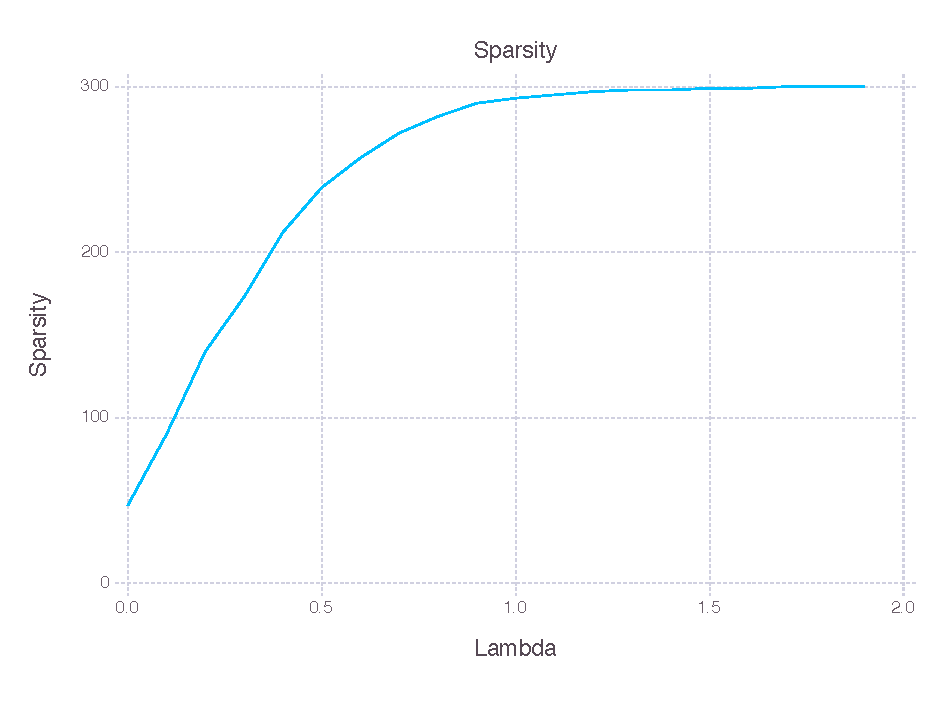
\includegraphics[width=\textwidth]{sparsityplotcount-20.pdf}
  \caption{A plot of the sparsity/shrinkage versus $\lambda$. The criteria for
    sparsity/shrinkage was the number of elements of $\beta_{est}$
    smaller than $10^{-3}$ when $\beta_{true}$ had 20 non-zero
    elements. The desired level of sparsity is reached at slightly
    below $\lambda = 1$.}
\label{fig:sparse20}
\end{subfigure}\\
\begin{subfigure}[b]{0.5\textwidth}
  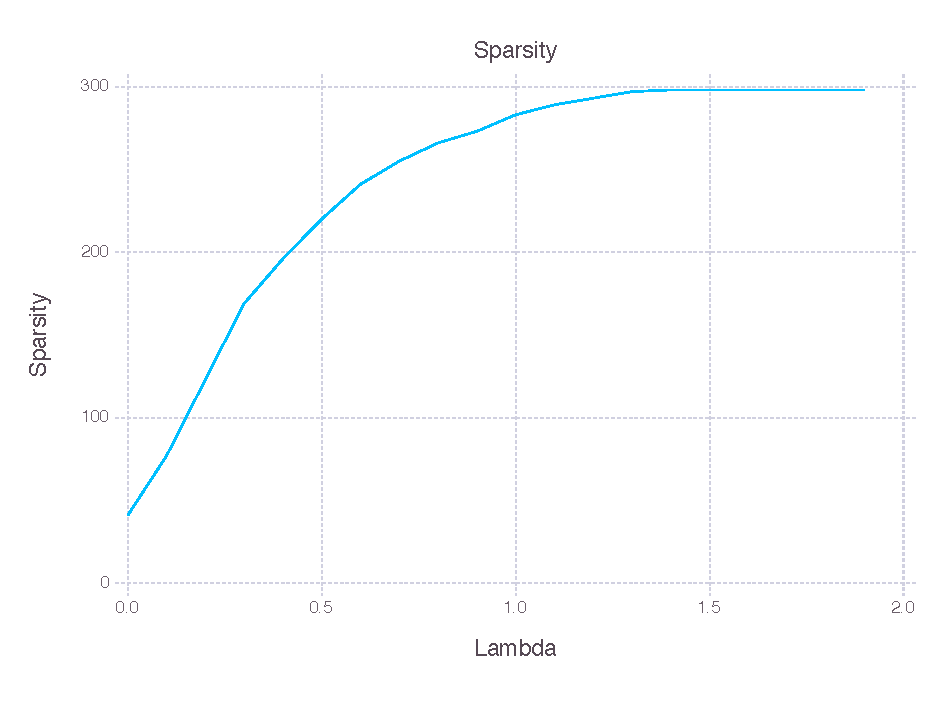
\includegraphics [width=\textwidth]{sparsityplotcount-75.pdf}
  \caption{A plot of the sparsity/shrinkage versus $\lambda$. The criteria for
    sparsity/shrinkage was the number of elements of $\beta_{est}$
    smaller than $10^{-3}$ when $\beta_{true}$ had 75 non-zero
    elements. The desired level of sparsity is reached at $\lambda = 0.5$.}
\label{fig:sparse75}
\end{subfigure}
        \caption{A plot of the sparsity/shrinkage versus $\lambda$. }\label{fig:sparse}
\end{figure}
\begin{figure}
\centering 
\begin{subfigure}[b]{0.5\textwidth}
  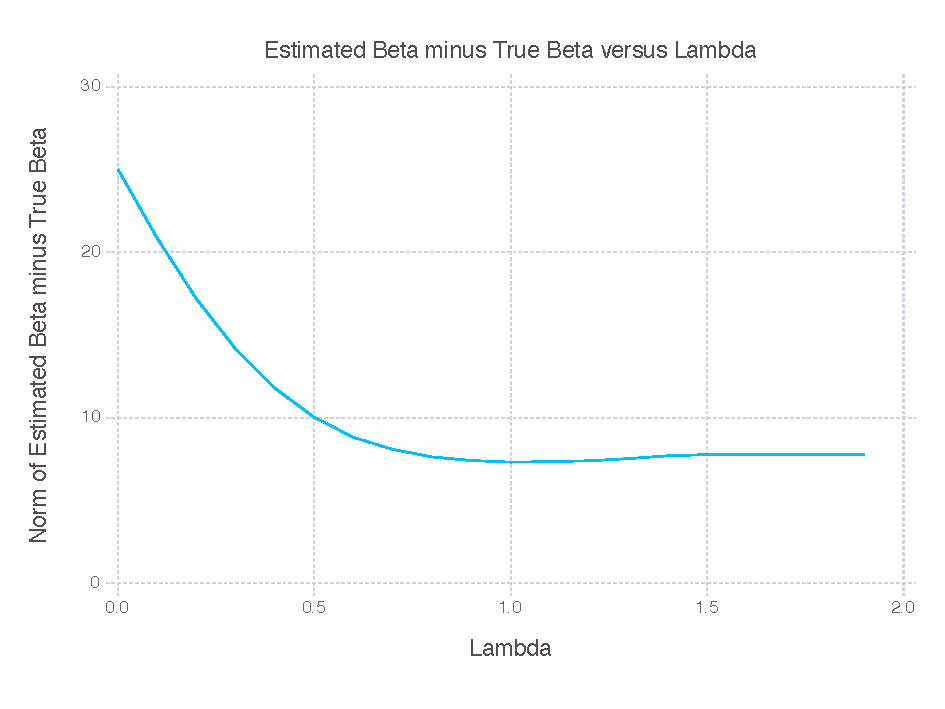
\includegraphics[width=\textwidth]{betaoptplotcount-20.pdf}
  \caption{A plot of the norm of $\beta_{true} -
    \beta_{est}$ versus $\lambda$ when $\beta_{true}$ had 20 non-zero
    elements. $\lambda = 1.0$ minimizes the norm.}
\label{fig:beta20}
\end{subfigure}\\
\begin{subfigure}[b]{0.5\textwidth}
  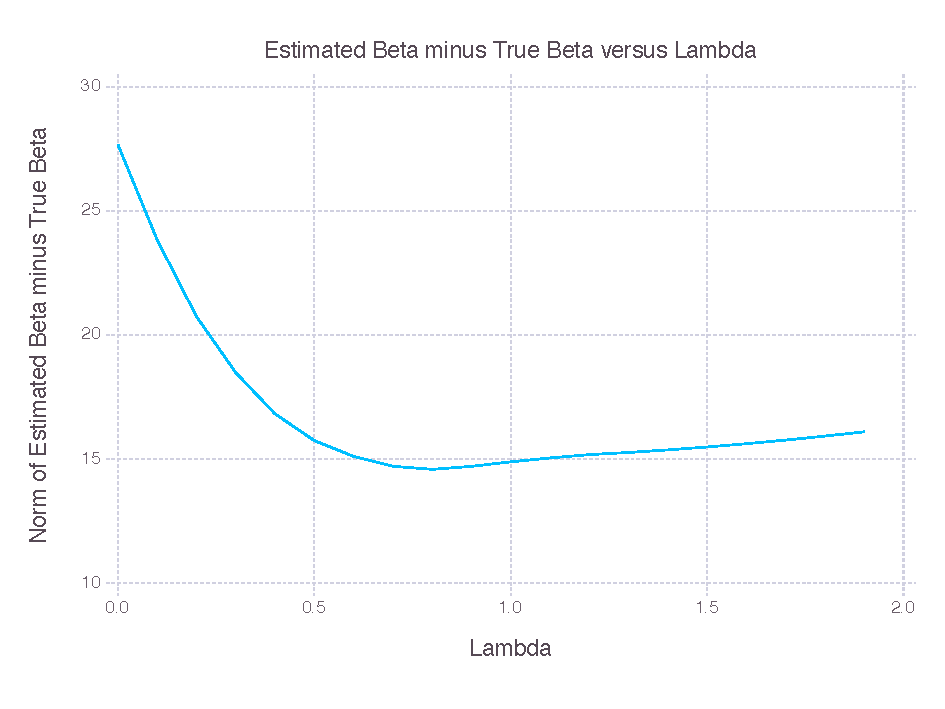
\includegraphics [width=\textwidth]{betaoptplotcount-75.pdf}
  \caption{A plot of the norm of $\beta_{true} -
    \beta_{est}$ versus $\lambda$ when $\beta_{true}$ had 75 non-zero
    elements. In this case it is clear that $\lambda = 0.7$ minimizes
    the norm.}
\label{fig:beta75}
\end{subfigure}
        \caption{A plot of the norm of $\beta_{true} -
    \beta_{est}$  versus $\lambda$. }\label{fig:sparse}
\end{figure}
\begin{figure}
\centering 
\begin{subfigure}[b]{0.5\textwidth}
  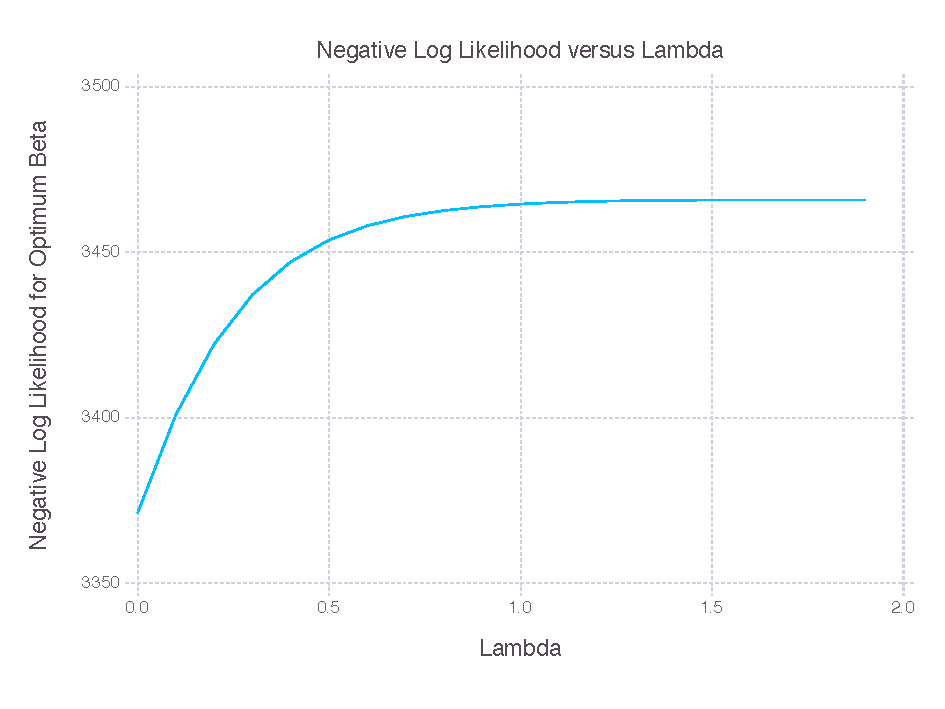
\includegraphics[width=\textwidth]{nlogoptplotcount-20.pdf}
  \caption{A plot of the negative log-likelihood versus $\lambda$ when
    $\beta_{true}$ had 20 non-zero elements. It seems to reach a
    maximum at $\lambda = 1.0$ and then stay at that level.}
\label{fig:nll20}
\end{subfigure}\\
\begin{subfigure}[b]{0.5\textwidth}
  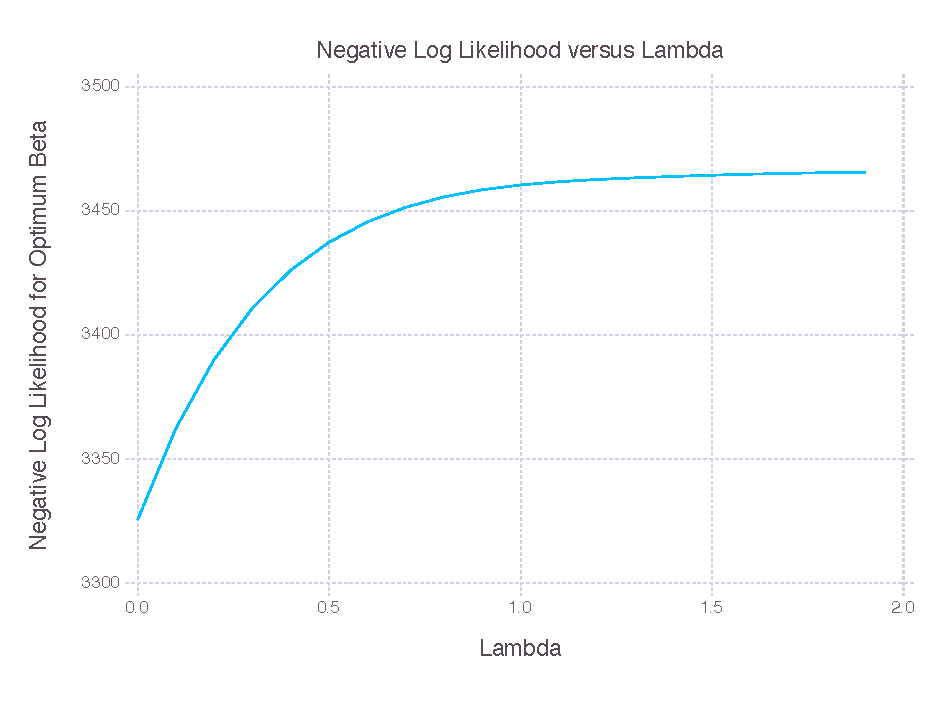
\includegraphics [width=\textwidth]{nlogoptplotcount-75.pdf}
  \caption{A plot of the negative log-likelihood versus $\lambda$ when
    $\beta_{true}$ had 75 non-zero elements. As in the case with 25
    non-zero elements, it seems to reach a
    maximum at $\lambda = 1.0$ and then increase at a very slow rate.}
\label{fig:nll75}
\end{subfigure}
        \caption{Negative log-likelihood versus $\lambda$. }\label{fig:sparse}
\end{figure}
\begin{figure}
\centering 
\begin{subfigure}[b]{0.4\textwidth}
                \includegraphics[width=\textwidth]{{errorcplot10-20.pdf}}
                \caption{Epsilon for $\lambda = 1$}
                \label{fig:errorc20}
        \end{subfigure}
\begin{subfigure}[b]{0.4\textwidth}
                \includegraphics[width=\textwidth]{{trueerrorplot10-20.pdf}}
                \caption{Norm of $\beta_{true} - \beta_{est}$ when $\lambda = 1$}
                \label{fig:true20}
        \end{subfigure}\\
\begin{subfigure}[b]{0.5\textwidth}
                \includegraphics[width=\textwidth]{{nllplot10-20.pdf}}
                \caption{Negative Log-likelihood when $\lambda = 1$}
                \label{fig:nll20}
        \end{subfigure}
        \caption{Plots for Subgradient Descent Algorithm with
          $\beta_{true}$ having 20 non-zero elements and $\lambda = 1$.}\label{fig:20}
\end{figure}
\begin{figure}
\centering 
\begin{subfigure}[b]{0.4\textwidth}
                \includegraphics[width=\textwidth]{{errorcplot10-20.pdf}}
                \caption{Epsilon for $\lambda = 0.8$}
                \label{fig:errorc20-8}
        \end{subfigure}
\begin{subfigure}[b]{0.4\textwidth}
                \includegraphics[width=\textwidth]{{trueerrorplot10-20.pdf}}
                \caption{Norm of $\beta_{true} - \beta_{est}$ when $\lambda = 0.8$}
                \label{fig:true20-8}
        \end{subfigure}\\
\begin{subfigure}[b]{0.5\textwidth}
                \includegraphics[width=\textwidth]{{nllplot10-20.pdf}}
                \caption{Negative Log-likelihood when $\lambda = 0.8$}
                \label{fig:nll20-8}
        \end{subfigure}
        \caption{Plots for Subgradient Descent Algorithm with
          $\beta_{true}$ having 20 non-zero elements and $\lambda = 0.8$.}\label{fig:20}
\end{figure}
\begin{figure}
\centering 
\begin{subfigure}[b]{0.4\textwidth}
                \includegraphics[width=\textwidth]{{errorcplot7-75.pdf}}
                \caption{Epsilon for $\lambda = 0.7$}
                \label{fig:errorc75}
        \end{subfigure}
\begin{subfigure}[b]{0.4\textwidth}
                \includegraphics[width=\textwidth]{{trueerrorplot7-75.pdf}}
                \caption{Norm of $\beta_{true} - \beta_{est}$ when $\lambda = 0.7$}
                \label{fig:true75}
        \end{subfigure}\\
\begin{subfigure}[b]{0.5\textwidth}
                \includegraphics[width=\textwidth]{{nllplot7-75.pdf}}
                \caption{Negative Log-likelihood when $\lambda = 0.7$}
                \label{fig:nll75}
        \end{subfigure}
        \caption{Plots for Subgradient Descent Algorithm with
          $\beta_{true}$ having 75 non-zero elements and $\lambda = 0.7$.}\label{fig:75}
\end{figure}

\begin{figure}
\centering 
\begin{subfigure}[b]{0.4\textwidth}
                \includegraphics[width=\textwidth]{{errorcplot5-75.pdf}}
                \caption{Epsilon for $\lambda = 0.7$}
                \label{fig:errorc75-5}
        \end{subfigure}
\begin{subfigure}[b]{0.4\textwidth}
                \includegraphics[width=\textwidth]{{trueerrorplot5-75.pdf}}
                \caption{Norm of $\beta_{true} - \beta_{est}$ when $\lambda = 0.7$}
                \label{fig:true75-5}
        \end{subfigure}\\
\begin{subfigure}[b]{0.5\textwidth}
                \includegraphics[width=\textwidth]{{nllplot5-75.pdf}}
                \caption{Negative Log-likelihood when $\lambda = 0.7$}
                \label{fig:nll75-5}
        \end{subfigure}
        \caption{Plots for Subgradient Descent Algorithm with
          $\beta_{true}$ having 75 non-zero elements and $\lambda = 0.5$.}\label{fig:75}
\end{figure}

\pagebreak 

\paragraph{Appendix:Julia code}
\begin{verbatim}
using PyPlot
using Distributions
using Gadfly


srand(12345)
print("enter p "); p = int(readline(STDIN))
print("enter n  "); n = int(readline(STDIN))
print("enter notsparse  "); notsparse = int(readline(STDIN))

function gradf(X::Matrix{Float64},y::Vector{Int}, 
p::Vector{Float64}, lambda::Float64,beta::Vector{Float64})
    -X'*(y-p)+lambda*sign(beta)
end

function neglogLkhd(probOld::Vector{Float64}, 
y::Vector{Int}, lambda::Float64, betaOld::Vector{Float64})
    n = length(y)
    z = zeros(n)
    p = length(betaOld)
    penaltyterm = zeros(p)
    for i = 1:n
            term1 = y[i]*log(probOld[i])
            term2 = (1-y[i])*log(1-probOld[i])
            z[i] = -term1-term2
        end
    	for i = 1:p
            penaltyterm[i] = lambda*abs(betaOld[i])
        end    
	(sum(z) + sum(penaltyterm))
end

expit(x::Float64) = exp(x)/(1+exp(x))
expit(V::Vector{Float64}) = [expit(v) for v in V]

rbern(p::Float64) = 0<p<1?rand(Bernoulli(p))
:error("p not in (0,1)")
rbern(V::Vector{Float64}) = [rbern(v) for v in V]

dataMat = rand(n,p)
(U,S,V) = svd(dataMat); @elapsed svd(dataMat)
#d = rand(Uniform(0,sqrt(30)),p)
#X = U*diagm(d)*V'
X = U*V'
betaTrue = rand(Normal(0,2),notsparse)
betaTrue =  [betaTrue;zeros((p-notsparse))]
Xbeta = X*betaTrue
probTrue = expit(Xbeta)
y = rbern(probTrue)

maxcount = 20
sparsityvec = zeros(maxcount)
for count = 1:maxcount
lambda = 0.1*count 
maxIter = 100000
betaOld = zeros(p)+1
Xbeta = X*betaOld
probOld = expit(Xbeta)
alpha = 1
tol = 10.0^-5
iter = 0
eps = 1
betamat = betaOld 
betaopt = betaOld
Xbeta = X*betaOld
probopt = expit(Xbeta)

neglogLkhdvec = neglogLkhd(probopt,y,lambda,betaopt)
epsvec = eps
trueerror = sqrt(dot(betaopt-betaTrue,betaopt-betaTrue))
trueerrorvec = trueerror

while iter< maxIter && eps > tol
	betaNew = betaOld - (alpha/(iter+1))*gradf(X,y,
probOld,lambda, betaOld)
	Xbeta = X*betaNew
    	probNew = expit(Xbeta)
    	eps = sqrt(dot(betaNew-betaopt,betaNew-betaopt))
	trueerror = sqrt(dot(betaopt-betaTrue,betaopt-betaTrue))

	if neglogLkhd(probNew,y,lambda,betaNew)
<neglogLkhd(probopt,y,lambda,betaopt)
           betaopt = betaNew
           Xbeta = X*betaopt
           probopt = expit(Xbeta)
        end

	betaOld = betaNew
	probOld = probNew

	if (iter%100) == 0
	   println("Iteration:",iter," " ,
neglogLkhd(probOld,y,lambda,betaOld)," ",eps,"\n")
	end
	   
	neglogLkhdvec = [neglogLkhdvec 
neglogLkhd(probopt,y,lambda,betaopt)]
	epsvec = [epsvec eps]
	trueerrorvec = [trueerrorvec trueerror]
	iter = iter+1
end
end
\end{verbatim}
\end{document}